\section{Part 1: ANDi Tool and Loopback}
\label{sec:andi-tool}

This chapter introduces the initial setup and basic testing procedures.

\subsection{Introduction to the ANDI-tool}
% Describe the ANDI-tool, its purpose, and main features.
ANDi (Automotive Network Diagnoser ) is a cross-platform test and analysis tool for automotive electronic networks, designed to support software and ECU development at every stage. Its core functions are to simulate network traffic, execute component tests and analyse the resulting data\cite{technica}. It supports simulation, monitoring, and analysis of various network protocols, including CAN, LIN, FlexRay, and Ethernet (BroadR-Reach).
   
\subsection{Introduction to Wireshark}
Wireshark is a widely used open-source network protocol analyser. Its primary purpose is to capture and inspect data packets travelling across a network, enabling detailed analysis of network traffic. Key features include real-time packet capture, deep inspection of hundreds of protocols, filtering capabilities, and the ability to reconstruct data streams. 
   
\subsection{Loopback Test Procedure}
% Explain the steps to perform a loopback test. You can use an itemize or enumerate environment.
\begin{itemize}
    \item Step 1: Connect the hardware: Attach the ANDi device to the CAN bus or network interface intended for testing, ensuring all physical connections are secure and correct. 
    \item Step 2: Configure the software: Launch the ANDi software, set up the interface parameters (bitrate, channel, etc.), and enable loopback mode in the configuration settings. 
    \item Step 3: Run the test and observe results: Start the loopback test, send messages through the interface, and monitor received frames to verify correct transmission and reception within the same device. 
\end{itemize}

\subsection{Task Report}
The task utilized the ANDi tool in combination with Wireshark to establish communication through loopback testing. To achieve this, a stimulation and a logging adapter had to be selected. The stimulation adapter should transmit frames or signals, while the logging adapter is used to receive incoming packets.\\\\
After running a loopback script included in the task the packages were captured as expected, but only after selecting the right adapter for both (Figure 1). The layer 2 frame was received as expected (Figure 2) and could be traced in Wireshark.\\\\
\begin{figure}[h]
    \centering
     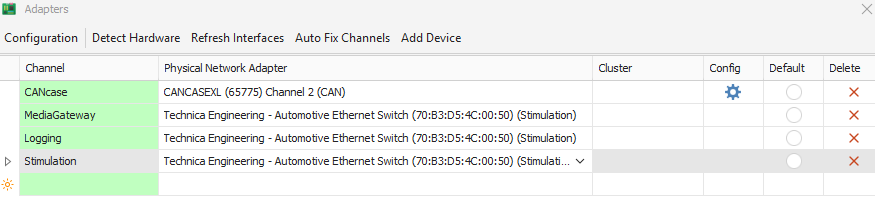
\includegraphics[width=0.8\textwidth]{figures/pictures/adaptersloopback.png}
    \caption{Selection of the same adapter for Logging and Stimulation.}
    \label{fig:mediagateway_setup}
\end{figure}
\begin{figure}[h]
    \centering
     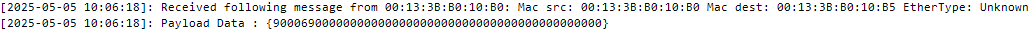
\includegraphics[width=0.8\textwidth]{figures/pictures/loopbackreceived.png}
    \caption{Received frame from loopback.}
    \label{fig:mediagateway_setup2}
\end{figure}
The next step was to create 2 distinct scripts, to distinguish between sending and receiving frames. Additionally the frames should be more distinguishable from another, so the requirement was to give each frame an identifier corresponding to the order they were sent in with 20 frames being sent over the course of 20 seconds.\\\\
After achieving this, subsequent task were to test further ANDi tools like SendPing and Burst Sending and analyze the traffic: Send Ping sends one request and awaits a reply while Burst Sending sends multiple requests in a short time without waiting for a reply first. Both operate on Layer 3 and use Ethernet frames on Layer 2 with the key difference being the number and timing of packets sent. \\\\
After changing the communication from Layer 2 (MAC address) to a layer 3 (IP address)  connection, the data frames change. They reveal more information about the connection, TTL, ports, and the checksum of the packages. 

\subsection{Conclusion}
In this package of Tasks basic understanding of packet construction and data traffic was developed by experimenting with a simulated point to point connection. The tasks were fairly basic and deepened the theoretical understanding of the topic, ensuring fundamental knowledge needed for subsequent tasks. No difficult challenges were encountered and the workflow was straightforward.

%To Do: Screenshots einfügen; 

